% Options for packages loaded elsewhere
\PassOptionsToPackage{unicode}{hyperref}
\PassOptionsToPackage{hyphens}{url}
\documentclass[
]{book}
\usepackage{xcolor}
\usepackage{amsmath,amssymb}
\setcounter{secnumdepth}{5}
\usepackage{iftex}
\ifPDFTeX
  \usepackage[T1]{fontenc}
  \usepackage[utf8]{inputenc}
  \usepackage{textcomp} % provide euro and other symbols
\else % if luatex or xetex
  \usepackage{unicode-math} % this also loads fontspec
  \defaultfontfeatures{Scale=MatchLowercase}
  \defaultfontfeatures[\rmfamily]{Ligatures=TeX,Scale=1}
\fi
\usepackage{lmodern}
\ifPDFTeX\else
  % xetex/luatex font selection
\fi
% Use upquote if available, for straight quotes in verbatim environments
\IfFileExists{upquote.sty}{\usepackage{upquote}}{}
\IfFileExists{microtype.sty}{% use microtype if available
  \usepackage[]{microtype}
  \UseMicrotypeSet[protrusion]{basicmath} % disable protrusion for tt fonts
}{}
\makeatletter
\@ifundefined{KOMAClassName}{% if non-KOMA class
  \IfFileExists{parskip.sty}{%
    \usepackage{parskip}
  }{% else
    \setlength{\parindent}{0pt}
    \setlength{\parskip}{6pt plus 2pt minus 1pt}}
}{% if KOMA class
  \KOMAoptions{parskip=half}}
\makeatother
\usepackage{color}
\usepackage{fancyvrb}
\newcommand{\VerbBar}{|}
\newcommand{\VERB}{\Verb[commandchars=\\\{\}]}
\DefineVerbatimEnvironment{Highlighting}{Verbatim}{commandchars=\\\{\}}
% Add ',fontsize=\small' for more characters per line
\usepackage{framed}
\definecolor{shadecolor}{RGB}{248,248,248}
\newenvironment{Shaded}{\begin{snugshade}}{\end{snugshade}}
\newcommand{\AlertTok}[1]{\textcolor[rgb]{0.94,0.16,0.16}{#1}}
\newcommand{\AnnotationTok}[1]{\textcolor[rgb]{0.56,0.35,0.01}{\textbf{\textit{#1}}}}
\newcommand{\AttributeTok}[1]{\textcolor[rgb]{0.13,0.29,0.53}{#1}}
\newcommand{\BaseNTok}[1]{\textcolor[rgb]{0.00,0.00,0.81}{#1}}
\newcommand{\BuiltInTok}[1]{#1}
\newcommand{\CharTok}[1]{\textcolor[rgb]{0.31,0.60,0.02}{#1}}
\newcommand{\CommentTok}[1]{\textcolor[rgb]{0.56,0.35,0.01}{\textit{#1}}}
\newcommand{\CommentVarTok}[1]{\textcolor[rgb]{0.56,0.35,0.01}{\textbf{\textit{#1}}}}
\newcommand{\ConstantTok}[1]{\textcolor[rgb]{0.56,0.35,0.01}{#1}}
\newcommand{\ControlFlowTok}[1]{\textcolor[rgb]{0.13,0.29,0.53}{\textbf{#1}}}
\newcommand{\DataTypeTok}[1]{\textcolor[rgb]{0.13,0.29,0.53}{#1}}
\newcommand{\DecValTok}[1]{\textcolor[rgb]{0.00,0.00,0.81}{#1}}
\newcommand{\DocumentationTok}[1]{\textcolor[rgb]{0.56,0.35,0.01}{\textbf{\textit{#1}}}}
\newcommand{\ErrorTok}[1]{\textcolor[rgb]{0.64,0.00,0.00}{\textbf{#1}}}
\newcommand{\ExtensionTok}[1]{#1}
\newcommand{\FloatTok}[1]{\textcolor[rgb]{0.00,0.00,0.81}{#1}}
\newcommand{\FunctionTok}[1]{\textcolor[rgb]{0.13,0.29,0.53}{\textbf{#1}}}
\newcommand{\ImportTok}[1]{#1}
\newcommand{\InformationTok}[1]{\textcolor[rgb]{0.56,0.35,0.01}{\textbf{\textit{#1}}}}
\newcommand{\KeywordTok}[1]{\textcolor[rgb]{0.13,0.29,0.53}{\textbf{#1}}}
\newcommand{\NormalTok}[1]{#1}
\newcommand{\OperatorTok}[1]{\textcolor[rgb]{0.81,0.36,0.00}{\textbf{#1}}}
\newcommand{\OtherTok}[1]{\textcolor[rgb]{0.56,0.35,0.01}{#1}}
\newcommand{\PreprocessorTok}[1]{\textcolor[rgb]{0.56,0.35,0.01}{\textit{#1}}}
\newcommand{\RegionMarkerTok}[1]{#1}
\newcommand{\SpecialCharTok}[1]{\textcolor[rgb]{0.81,0.36,0.00}{\textbf{#1}}}
\newcommand{\SpecialStringTok}[1]{\textcolor[rgb]{0.31,0.60,0.02}{#1}}
\newcommand{\StringTok}[1]{\textcolor[rgb]{0.31,0.60,0.02}{#1}}
\newcommand{\VariableTok}[1]{\textcolor[rgb]{0.00,0.00,0.00}{#1}}
\newcommand{\VerbatimStringTok}[1]{\textcolor[rgb]{0.31,0.60,0.02}{#1}}
\newcommand{\WarningTok}[1]{\textcolor[rgb]{0.56,0.35,0.01}{\textbf{\textit{#1}}}}
\usepackage{longtable,booktabs,array}
\usepackage{calc} % for calculating minipage widths
% Correct order of tables after \paragraph or \subparagraph
\usepackage{etoolbox}
\makeatletter
\patchcmd\longtable{\par}{\if@noskipsec\mbox{}\fi\par}{}{}
\makeatother
% Allow footnotes in longtable head/foot
\IfFileExists{footnotehyper.sty}{\usepackage{footnotehyper}}{\usepackage{footnote}}
\makesavenoteenv{longtable}
\usepackage{graphicx}
\makeatletter
\newsavebox\pandoc@box
\newcommand*\pandocbounded[1]{% scales image to fit in text height/width
  \sbox\pandoc@box{#1}%
  \Gscale@div\@tempa{\textheight}{\dimexpr\ht\pandoc@box+\dp\pandoc@box\relax}%
  \Gscale@div\@tempb{\linewidth}{\wd\pandoc@box}%
  \ifdim\@tempb\p@<\@tempa\p@\let\@tempa\@tempb\fi% select the smaller of both
  \ifdim\@tempa\p@<\p@\scalebox{\@tempa}{\usebox\pandoc@box}%
  \else\usebox{\pandoc@box}%
  \fi%
}
% Set default figure placement to htbp
\def\fps@figure{htbp}
\makeatother
\setlength{\emergencystretch}{3em} % prevent overfull lines
\providecommand{\tightlist}{%
  \setlength{\itemsep}{0pt}\setlength{\parskip}{0pt}}
\usepackage[]{natbib}
\bibliographystyle{apalike}
\usepackage{bookmark}
\IfFileExists{xurl.sty}{\usepackage{xurl}}{} % add URL line breaks if available
\urlstyle{same}
\hypersetup{
  pdftitle={Writing GitBooks Tutorial},
  pdfauthor={Ville Langén},
  hidelinks,
  pdfcreator={LaTeX via pandoc}}

\title{Writing GitBooks Tutorial}
\author{Ville Langén}
\date{2025-07-10}

\begin{document}
\maketitle

{
\setcounter{tocdepth}{1}
\tableofcontents
}
\chapter*{Preface}\label{preface}
\addcontentsline{toc}{chapter}{Preface}

This is a tutorial about making tutorials in GitBook format using RStudio and bookdown.

Whether you're a data scientist, researcher, or educator, creating beautiful, interactive tutorials and documentation is essential for sharing your knowledge effectively. This guide will walk you through the entire process of creating professional-looking GitBook-style tutorials using R, RStudio, and the powerful bookdown package.

\textbf{The method we'll be covering is so powerful that it not only creates a web page but also generates an EPUB e-book and a PDF document automatically!} This very e-book is also released in EPUB and PDF formats:

\textbf{\href{writing-gitbooks-tutorial.epub}{EPUB format}} - Perfect for e-readers and mobile devices\\
\textbf{\href{writing-gitbooks-tutorial.pdf}{PDF format}} - Print-ready professional document

All three formats are generated from the same source files with a single command!

\section*{What You'll Learn}\label{what-youll-learn}
\addcontentsline{toc}{section}{What You'll Learn}

\begin{itemize}
\tightlist
\item
  How to set up your development environment
\item
  Understanding the GitBook format and bookdown
\item
  Writing effective tutorial content with R Markdown
\item
  Publishing your tutorials online
\end{itemize}

\section*{Prerequisites}\label{prerequisites}
\addcontentsline{toc}{section}{Prerequisites}

Basic familiarity with R and R Markdown is helpful but not required. We'll guide you through everything step by step.

\chapter{Introduction to GitBook Format}\label{intro}

\section{What is GitBook Format?}\label{what-is-gitbook-format}

GitBook is a modern documentation format that creates beautiful, interactive books and tutorials from Markdown files. Originally developed as a platform for writing and publishing books, the GitBook format has become popular for:

\begin{itemize}
\tightlist
\item
  Technical documentation
\item
  API guides
\item
  Educational tutorials
\item
  Research papers
\item
  Software manuals
\end{itemize}

The format features:

\begin{itemize}
\tightlist
\item
  \textbf{Clean, responsive design} that works on desktop and mobile
\item
  \textbf{Interactive navigation} with a collapsible table of contents
\item
  \textbf{Search functionality} built-in
\item
  \textbf{Code syntax highlighting}
\item
  \textbf{Mathematical equations} support
\item
  \textbf{Cross-references} and internal linking
\end{itemize}

\section{What is bookdown::gitbook?}\label{what-is-bookdowngitbook}

\texttt{bookdown::gitbook} is an R package output format that creates GitBook-style HTML books from R Markdown files. It's part of the \texttt{bookdown} package ecosystem created by Yihui Xie.

Key features of \texttt{bookdown::gitbook}:

\begin{itemize}
\tightlist
\item
  \textbf{Multi-chapter books} from multiple .Rmd files
\item
  \textbf{Automatic cross-referencing} of figures, tables, and sections
\item
  \textbf{Citation management} with BibTeX
\item
  \textbf{Code chunk execution} with live R output
\item
  \textbf{Mathematical notation} with LaTeX syntax
\item
  \textbf{Customizable themes} and styling
\end{itemize}

\section{Real-World Examples}\label{real-world-examples}

Here are some excellent examples of GitBook-style tutorials and documentation:

\subsection{Data Science}\label{data-science}

\begin{itemize}
\tightlist
\item
  \href{https://r4ds.had.co.nz/}{R for Data Science} by Hadley Wickham
\item
  \href{https://adv-r.hadley.nz/}{Advanced R} by Hadley Wickham
\item
  \href{https://www.tmwr.org/}{Tidy Modeling with R} by Max Kuhn and Julia Silge
\end{itemize}

\subsection{Statistics and Research}\label{statistics-and-research}

\begin{itemize}
\tightlist
\item
  \href{https://moderndive.com/}{Statistical Inference via Data Science} by Chester Ismay
\item
  \href{https://geocompr.robinlovelace.net/}{Geocomputation with R} by Robin Lovelace
\end{itemize}

\subsection{Web Development}\label{web-development}

\begin{itemize}
\tightlist
\item
  \href{https://engineering-shiny.org/}{Engineering Production-Grade Shiny Apps}
\item
  \href{https://mastering-shiny.org/}{Mastering Shiny} by Hadley Wickham
\end{itemize}

These examples demonstrate the power and versatility of the GitBook format for creating comprehensive, professional documentation that's both beautiful and functional.

\chapter{Installation and Setup}\label{install}

Before we can start creating GitBook tutorials, we need to set up our development environment. This chapter will guide you through installing all the necessary tools.

\section{Installing R}\label{installing-r}

R is the foundation of our toolkit. It's a free, open-source programming language specifically designed for statistical computing and graphics.

\subsection{Download and Install R}\label{download-and-install-r}

\begin{enumerate}
\def\labelenumi{\arabic{enumi}.}
\tightlist
\item
  Visit the official R website: \url{https://cran.r-project.org}
\item
  Click on ``Download R for your operating system''
\item
  Choose a mirror close to your location
\item
  Download the latest version of R
\item
  Run the installer and follow the installation wizard
\end{enumerate}

\subsection{Verify R Installation}\label{verify-r-installation}

Open your terminal or command prompt and type:

\begin{Shaded}
\begin{Highlighting}[]
\ExtensionTok{R} \AttributeTok{{-}{-}version}
\end{Highlighting}
\end{Shaded}

You should see output showing the R version number.

\section{Installing RStudio}\label{installing-rstudio}

RStudio is an integrated development environment (IDE) that makes working with R much more pleasant and productive.

\subsection{Download and Install RStudio}\label{download-and-install-rstudio}

\begin{enumerate}
\def\labelenumi{\arabic{enumi}.}
\tightlist
\item
  Visit: \url{https://posit.co/download/rstudio-desktop/}
\item
  Download RStudio Desktop (free version)
\item
  Run the installer appropriate for your operating system
\item
  Launch RStudio to verify it works
\end{enumerate}

\subsection{First Launch}\label{first-launch}

When you first open RStudio, you'll see four panes:
- \textbf{Console} (bottom left): Where R commands are executed
- \textbf{Environment} (top right): Shows your variables and data
- \textbf{Files/Plots/Help} (bottom right): File browser and output
- \textbf{Editor} (top left): Where you'll write your .Rmd files

\section{Installing Git}\label{installing-git}

Git is essential for version control and publishing your tutorials online.

\subsection{Download and Install Git}\label{download-and-install-git}

Visit \url{https://git-scm.com/} and download Git for your operating system.

\subsubsection{Windows}\label{windows}

\begin{itemize}
\tightlist
\item
  Download Git for Windows
\item
  Run the installer with default settings
\end{itemize}

\subsubsection{macOS}\label{macos}

\begin{itemize}
\tightlist
\item
  Git comes pre-installed on most Mac systems
\item
  Alternatively, install via Homebrew: \texttt{brew\ install\ git}
\end{itemize}

\subsubsection{Linux}\label{linux}

\begin{itemize}
\tightlist
\item
  Ubuntu/Debian: \texttt{sudo\ apt-get\ install\ git}
\item
  CentOS/RHEL: \texttt{sudo\ yum\ install\ git}
\end{itemize}

\subsection{Configure Git}\label{configure-git}

Set up your identity (replace with your information):

\begin{Shaded}
\begin{Highlighting}[]
\FunctionTok{git}\NormalTok{ config }\AttributeTok{{-}{-}global}\NormalTok{ user.name }\StringTok{"Your Name"}
\FunctionTok{git}\NormalTok{ config }\AttributeTok{{-}{-}global}\NormalTok{ user.email }\StringTok{"your.email@example.com"}
\end{Highlighting}
\end{Shaded}

\section{Installing R Packages}\label{installing-r-packages}

Now we'll install the R packages needed for creating GitBooks.

\subsection{Essential Packages}\label{essential-packages}

Open RStudio and run these commands in the Console:

\begin{Shaded}
\begin{Highlighting}[]
\CommentTok{\# Install the main package}
\FunctionTok{install.packages}\NormalTok{(}\StringTok{"bookdown"}\NormalTok{)}

\CommentTok{\# Install supporting packages}
\FunctionTok{install.packages}\NormalTok{(}\FunctionTok{c}\NormalTok{(}\StringTok{"rmarkdown"}\NormalTok{, }\StringTok{"knitr"}\NormalTok{))}
\end{Highlighting}
\end{Shaded}

\subsection{Optional but Recommended Packages}\label{optional-but-recommended-packages}

These packages will enhance your GitBook creation experience:

\begin{Shaded}
\begin{Highlighting}[]
\CommentTok{\# For better plots and data manipulation}
\FunctionTok{install.packages}\NormalTok{(}\FunctionTok{c}\NormalTok{(}\StringTok{"ggplot2"}\NormalTok{, }\StringTok{"dplyr"}\NormalTok{, }\StringTok{"tidyr"}\NormalTok{))}

\CommentTok{\# For web publishing}
\FunctionTok{install.packages}\NormalTok{(}\StringTok{"servr"}\NormalTok{)}

\CommentTok{\# For advanced formatting}
\FunctionTok{install.packages}\NormalTok{(}\FunctionTok{c}\NormalTok{(}\StringTok{"DT"}\NormalTok{, }\StringTok{"htmlwidgets"}\NormalTok{))}
\end{Highlighting}
\end{Shaded}

\subsection{Verify Package Installation}\label{verify-package-installation}

Test that bookdown is working:

\begin{Shaded}
\begin{Highlighting}[]
\FunctionTok{library}\NormalTok{(bookdown)}
\FunctionTok{packageVersion}\NormalTok{(}\StringTok{"bookdown"}\NormalTok{)}
\end{Highlighting}
\end{Shaded}

\section{Create Your First Project}\label{create-your-first-project}

Let's verify everything is working by creating a test project:

\begin{enumerate}
\def\labelenumi{\arabic{enumi}.}
\tightlist
\item
  In RStudio, go to \textbf{File \textgreater{} New Project \textgreater{} New Directory}
\item
  Choose \textbf{Book Project using bookdown}
\item
  Give it a name like ``test-gitbook''
\item
  Click \textbf{Create Project}
\end{enumerate}

RStudio will create a sample bookdown project with example files. You can render it by running:

\begin{Shaded}
\begin{Highlighting}[]
\NormalTok{bookdown}\SpecialCharTok{::}\FunctionTok{render\_book}\NormalTok{(}\StringTok{"index.Rmd"}\NormalTok{)}
\end{Highlighting}
\end{Shaded}

If everything is installed correctly, this will generate a GitBook in the \texttt{\_book/} folder!

\section{Troubleshooting}\label{troubleshooting}

\subsection{Common Issues}\label{common-issues}

\textbf{Issue}: ``Package `bookdown' not found''
- \textbf{Solution}: Make sure you've installed the package: \texttt{install.packages("bookdown")}

\textbf{Issue}: Git not recognized
- \textbf{Solution}: Restart RStudio after installing Git, or add Git to your system PATH

\textbf{Issue}: LaTeX errors when rendering
- \textbf{Solution}: Install TinyTeX: \texttt{tinytex::install\_tinytex()}

\subsection{Getting Help}\label{getting-help}

\begin{itemize}
\tightlist
\item
  \textbf{R Documentation}: Use \texttt{?function\_name} in R console
\item
  \textbf{Bookdown Guide}: \url{https://bookdown.org/yihui/bookdown/}
\item
  \textbf{RStudio Community}: \url{https://community.rstudio.com/}
\end{itemize}

Congratulations! You now have a complete development environment for creating GitBook tutorials.

\chapter{Writing Tutorial Content}\label{content}

Now that you have your environment set up, let's learn how to create compelling tutorial content using R Markdown. This chapter covers the essential techniques for writing effective GitBook tutorials.

\section{Project Structure with .Rmd Files}\label{project-structure-with-.rmd-files}

Each \texttt{.Rmd} file in your project becomes a chapter in your GitBook. The structure is simple:

\begin{verbatim}
my-tutorial/
|-- index.Rmd          # Main page (Chapter 0)
|-- 01-chapter1.Rmd    # Chapter 1
|-- 02-chapter2.Rmd    # Chapter 2
|-- 03-chapter3.Rmd    # Chapter 3
`-- ...
\end{verbatim}

\subsection{File Naming Convention}\label{file-naming-convention}

\begin{itemize}
\tightlist
\item
  \textbf{index.Rmd}: Always the main/first page
\item
  \textbf{01-intro.Rmd}: Use numbers for ordering
\item
  \textbf{XY-descriptive-names.Rmd}: Use descriptive names after numbers
\end{itemize}

\section{Headings Create Sections}\label{headings-create-sections}

Headings automatically create your table of contents and navigation structure:

\begin{Shaded}
\begin{Highlighting}[]
\FunctionTok{\# Chapter Title \{\#chapter{-}id\}}

\FunctionTok{\#\# Main Section}

\FunctionTok{\#\#\# Subsection  }

\FunctionTok{\#\#\#\# Sub{-}subsection}
\end{Highlighting}
\end{Shaded}

\subsection{Important Notes:}\label{important-notes}

\begin{itemize}
\tightlist
\item
  \texttt{\#\ Chapter\ Title} creates a new chapter
\item
  \texttt{\{\#chapter-id\}} creates an ID for cross-referencing
\item
  Only use \texttt{\#} for chapter titles in chapter files
\item
  Use \texttt{\#\#}, \texttt{\#\#\#}, \texttt{\#\#\#\#} for sections within chapters
\end{itemize}

\section{Code Chunks: The Heart of R Tutorials}\label{code-chunks-the-heart-of-r-tutorials}

Code chunks are what make R Markdown special. They execute R code and display the results:

\subsection{Basic Code Chunk}\label{basic-code-chunk}

\begin{verbatim}
```{r}
# This is R code
x <- c(1, 2, 3, 4, 5)
mean(x)
```
\end{verbatim}

\begin{verbatim}
## [1] 3
\end{verbatim}

\subsection{Code Chunk Options}\label{code-chunk-options}

Control how your code appears and executes:

\begin{verbatim}
```{r your-chunk-name, echo=TRUE, eval=TRUE, fig.cap="Simple Line Plot"}
# echo=TRUE: Show the code
# eval=TRUE: Run the code  
# fig.cap: Caption for figures
plot(1:10, 1:10)
```
\end{verbatim}

Here's the actual chunk in action:

\begin{figure}
\centering
\pandocbounded{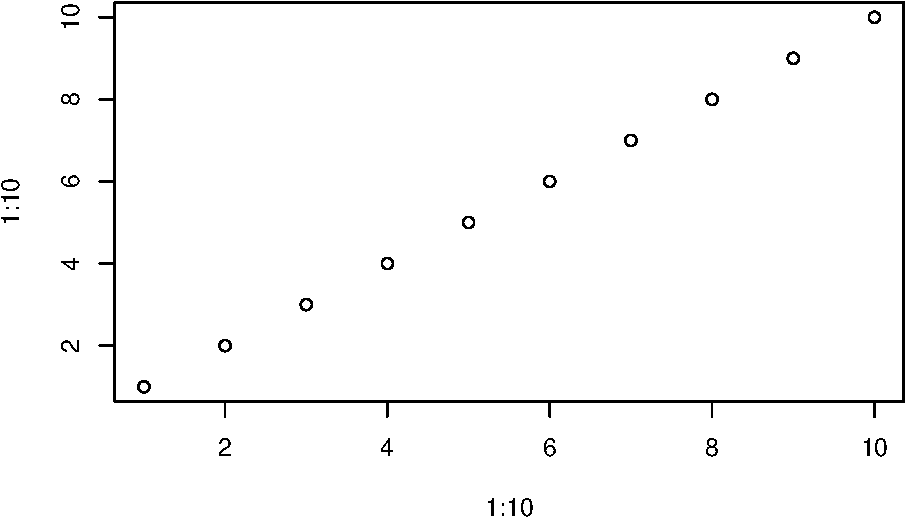
\includegraphics[keepaspectratio,alt={\label{fig:chunk-name}Simple Line Plot}]{writing-gitbooks-tutorial_files/figure-latex/chunk-name-1.pdf}}
\caption{\label{fig:chunk-name}Simple Line Plot}
\end{figure}

\textbf{Common options:}

\begin{itemize}
\tightlist
\item
  \texttt{echo=FALSE}: Hide code, show output
\item
  \texttt{eval=FALSE}: Show code, don't run it
\item
  \texttt{include=FALSE}: Run code, don't show anything
\item
  \texttt{message=FALSE}: Hide messages
\item
  \texttt{warning=FALSE}: Hide warnings
\end{itemize}

\section{Creating Plots and Visualizations}\label{creating-plots-and-visualizations}

R excels at creating beautiful plots:

\begin{Shaded}
\begin{Highlighting}[]
\FunctionTok{library}\NormalTok{(ggplot2)}
\FunctionTok{data}\NormalTok{(mtcars)}

\FunctionTok{ggplot}\NormalTok{(mtcars, }\FunctionTok{aes}\NormalTok{(}\AttributeTok{x =}\NormalTok{ mpg, }\AttributeTok{y =}\NormalTok{ hp)) }\SpecialCharTok{+}
  \FunctionTok{geom\_point}\NormalTok{(}\FunctionTok{aes}\NormalTok{(}\AttributeTok{color =} \FunctionTok{factor}\NormalTok{(cyl))) }\SpecialCharTok{+}
  \FunctionTok{labs}\NormalTok{(}\AttributeTok{title =} \StringTok{"Horsepower vs MPG"}\NormalTok{,}
       \AttributeTok{x =} \StringTok{"Miles per Gallon"}\NormalTok{,}
       \AttributeTok{y =} \StringTok{"Horsepower"}\NormalTok{,}
       \AttributeTok{color =} \StringTok{"Cylinders"}\NormalTok{) }\SpecialCharTok{+}
  \FunctionTok{theme\_minimal}\NormalTok{()}
\end{Highlighting}
\end{Shaded}

\begin{figure}
\centering
\pandocbounded{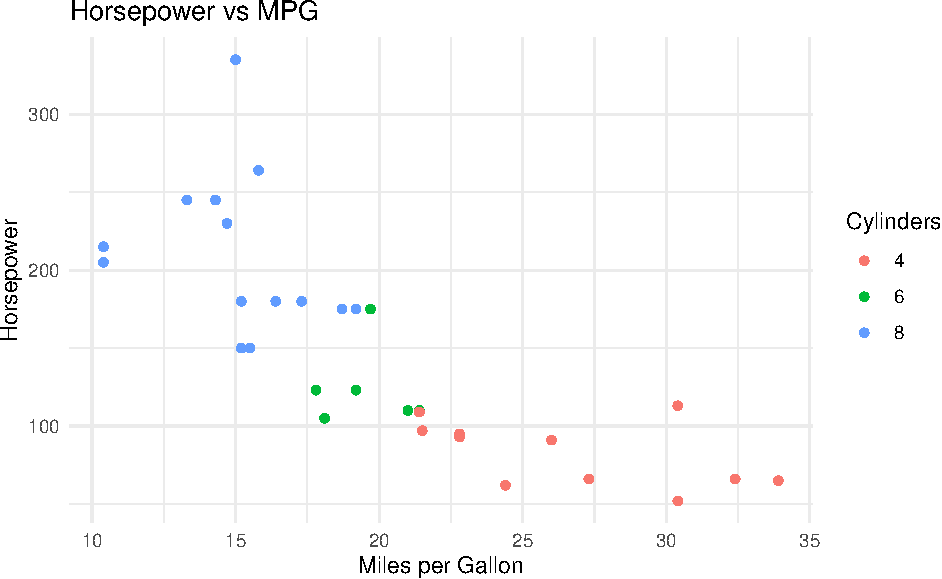
\includegraphics[keepaspectratio,alt={\label{fig:plot-example}Sample Scatter Plot}]{writing-gitbooks-tutorial_files/figure-latex/plot-example-1.pdf}}
\caption{\label{fig:plot-example}Sample Scatter Plot}
\end{figure}

\section{Inline R Code}\label{inline-r-code}

You can embed R results directly in your text using inline code:

The mean of \texttt{mtcars\$mpg} is \texttt{r\ round(mean(mtcars\$mpg),\ 2)} miles per gallon.

The mean of mtcars\$mpg is 20.09 miles per gallon.

\section{Mathematical Notation}\label{mathematical-notation}

LaTeX syntax works beautifully in GitBooks:

\subsection{Inline Math}\label{inline-math}

\begin{Shaded}
\begin{Highlighting}[]
\NormalTok{The formula is $y = mx + b$ where $m$ is the slope.}
\end{Highlighting}
\end{Shaded}

\textbf{Result:} The formula is \(y = mx + b\) where \(m\) is the slope.

\subsection{Block Math}\label{block-math}

\begin{Shaded}
\begin{Highlighting}[]
\NormalTok{$$}
\NormalTok{\textbackslash{}bar\{x\} = \textbackslash{}frac\{1\}\{n\} \textbackslash{}sum\_\{i=1\}\^{}\{n\} x\_i}
\NormalTok{$$}
\end{Highlighting}
\end{Shaded}

\textbf{Result:}
\[
\bar{x} = \frac{1}{n} \sum_{i=1}^{n} x_i
\]

\section{Cross-References and Links}\label{cross-references-and-links}

\subsection{Referencing Figures and Tables}\label{referencing-figures-and-tables}

\begin{Shaded}
\begin{Highlighting}[]
\NormalTok{See Figure \textbackslash{}@ref(fig:plot{-}example) for the scatter plot.}
\end{Highlighting}
\end{Shaded}

\textbf{Result:} See Figure \ref{fig:plot-example} for the scatter plot.

\subsection{Referencing Sections}\label{referencing-sections}

\begin{Shaded}
\begin{Highlighting}[]
\NormalTok{As we learned in Chapter \textbackslash{}@ref(intro), GitBook format is powerful.}
\end{Highlighting}
\end{Shaded}

\textbf{Result:} As we learned in Chapter \ref{intro}, GitBook format is powerful.

\subsection{Creating Tables}\label{creating-tables}

\begin{Shaded}
\begin{Highlighting}[]
\NormalTok{knitr}\SpecialCharTok{::}\FunctionTok{kable}\NormalTok{(}
  \FunctionTok{head}\NormalTok{(mtcars[, }\DecValTok{1}\SpecialCharTok{:}\DecValTok{4}\NormalTok{]), }
  \AttributeTok{caption =} \StringTok{"First few rows of mtcars dataset"}\NormalTok{,}
  \AttributeTok{booktabs =} \ConstantTok{TRUE}
\NormalTok{)}
\end{Highlighting}
\end{Shaded}

\begin{table}

\caption{\label{tab:cars-table}First few rows of mtcars dataset}
\centering
\begin{tabular}[t]{lrrrr}
\toprule
  & mpg & cyl & disp & hp\\
\midrule
Mazda RX4 & 21.0 & 6 & 160 & 110\\
Mazda RX4 Wag & 21.0 & 6 & 160 & 110\\
Datsun 710 & 22.8 & 4 & 108 & 93\\
Hornet 4 Drive & 21.4 & 6 & 258 & 110\\
Hornet Sportabout & 18.7 & 8 & 360 & 175\\
\addlinespace
Valiant & 18.1 & 6 & 225 & 105\\
\bottomrule
\end{tabular}
\end{table}

Reference it with: \texttt{Table\ \textbackslash{}@ref(tab:cars-table)}

\section{Optional Enhancements}\label{optional-enhancements}

\subsection{Footnotes}\label{footnotes}

Add footnotes for additional information. First, reference the footnote, then define what the footnote reads.
Footnotes will be placed at the bottom of the page automatically.

\begin{Shaded}
\begin{Highlighting}[]
\NormalTok{This is the text where the footnote is referenced}\OtherTok{[\^{}note1]}\NormalTok{.}
\OtherTok{[\^{}note1]: }\NormalTok{This is the content of the footnote.}
\end{Highlighting}
\end{Shaded}

Result:

This is the text where the footnote is referenced\footnote{And this is the content of the footnote.}.

(Scroll to the bottom of the page to see the footnote.)

\subsection{Citations with BibTeX}\label{citations-with-bibtex}

First, create a \texttt{references.bib} file:

\begin{Shaded}
\begin{Highlighting}[]
\VariableTok{@book}\NormalTok{\{}\OtherTok{wickham2016r}\NormalTok{,}
  \DataTypeTok{title}\NormalTok{=\{R for data science: import, tidy, transform, visualize, and model data\},}
  \DataTypeTok{author}\NormalTok{=\{Wickham, Hadley and Grolemund, Garrett\},}
  \DataTypeTok{year}\NormalTok{=\{2016\},}
  \DataTypeTok{publisher}\NormalTok{=\{O\textquotesingle{}Reilly Media\}}
\NormalTok{\}}
\end{Highlighting}
\end{Shaded}

Then cite it:

\begin{Shaded}
\begin{Highlighting}[]
\NormalTok{According to @wickham2016r, data science is a powerful approach.}
\end{Highlighting}
\end{Shaded}

\subsection{Adding Images}\label{adding-images}

\begin{Shaded}
\begin{Highlighting}[]
\AlertTok{![Caption for image](path/to/image.png)}
\end{Highlighting}
\end{Shaded}

Or with more control:

\begin{verbatim}
```{r, fig.cap="My Image", out.width="50%", eval=FALSE}
knitr::include_graphics("path/to/image.png")
```
\end{verbatim}

\subsection{Callouts and Special Blocks}\label{callouts-and-special-blocks}

Create attention-grabbing callouts:

\begin{Shaded}
\begin{Highlighting}[]
\AttributeTok{\textgreater{} **Note:** This is an important note that readers should pay attention to.}

\AttributeTok{\textgreater{} **Warning:** Be careful with this command as it might delete files.}

\AttributeTok{\textgreater{} **Tip:** Here\textquotesingle{}s a helpful tip to make your work easier.}
\end{Highlighting}
\end{Shaded}

\textbf{Results:}

\begin{quote}
\textbf{Note:} This is an important note that readers should pay attention to.
\end{quote}

\begin{quote}
\textbf{Warning:} Be careful with this command as it might delete files.
\end{quote}

\begin{quote}
\textbf{Tip:} Here's a helpful tip to make your work easier.
\end{quote}

\chapter{Publishing Your GitBook}\label{publish}

Once you've written your tutorial content, it's time to render and publish your GitBook. This chapter covers both local rendering for testing and online publishing for sharing with the world.

\section{Rendering Locally}\label{rendering-locally}

Local rendering lets you preview your GitBook before publishing. This is essential for testing and debugging.

\subsection{Basic Rendering Command}\label{basic-rendering-command}

The fundamental command to render your GitBook:

\begin{Shaded}
\begin{Highlighting}[]
\NormalTok{bookdown}\SpecialCharTok{::}\FunctionTok{render\_book}\NormalTok{(}\StringTok{"index.Rmd"}\NormalTok{, }\StringTok{"bookdown::gitbook"}\NormalTok{)}
\end{Highlighting}
\end{Shaded}

This command:
1. Processes all your .Rmd files in order
2. Executes all R code chunks
3. Generates HTML files in the \texttt{\_book/} directory
4. Creates navigation and cross-references

\subsection{Alternative Rendering Methods}\label{alternative-rendering-methods}

\subsubsection{Using RStudio Build Tab}\label{using-rstudio-build-tab}

\begin{enumerate}
\def\labelenumi{\arabic{enumi}.}
\tightlist
\item
  Open your project in RStudio
\item
  Go to the \textbf{Build} tab (usually in the top-right pane)
\item
  Click \textbf{Build Book}
\item
  Select \textbf{bookdown::gitbook}
\end{enumerate}

\subsubsection{Using the Knit Button}\label{using-the-knit-button}

\begin{itemize}
\tightlist
\item
  Open \texttt{index.Rmd}
\item
  Click the \textbf{Knit} dropdown
\item
  Select \textbf{Knit Book}
\end{itemize}

\subsection{Previewing Your Book}\label{previewing-your-book}

After rendering, you can preview your book:

\begin{Shaded}
\begin{Highlighting}[]
\CommentTok{\# Open the book in your browser}
\NormalTok{servr}\SpecialCharTok{::}\FunctionTok{httw}\NormalTok{(}\StringTok{"\_book"}\NormalTok{)}
\end{Highlighting}
\end{Shaded}

Or simply open \texttt{\_book/index.html} in your web browser --- my preferred method, every time.

\subsection{Multiple Output Formats}\label{multiple-output-formats}

You can render to multiple formats simultaneously:

\begin{Shaded}
\begin{Highlighting}[]
\CommentTok{\# Render GitBook, PDF, and EPUB}
\NormalTok{bookdown}\SpecialCharTok{::}\FunctionTok{render\_book}\NormalTok{(}\StringTok{"index.Rmd"}\NormalTok{, }\StringTok{"all"}\NormalTok{)}
\end{Highlighting}
\end{Shaded}

Common formats:
- \texttt{"bookdown::gitbook"}: Interactive HTML
- \texttt{"bookdown::pdf\_book"}: PDF document
- \texttt{"bookdown::epub\_book"}: EPUB e-book
- \texttt{"bookdown::word\_document2"}: Word document

\section{Publishing Online with GitHub + Netlify}\label{publishing-online-with-github-netlify}

The most reliable method: build locally, push to GitHub, deploy with Netlify.

\subsection{Step 1: Build Your Book Locally}\label{step-1-build-your-book-locally}

First, render your book on your local machine:

\begin{Shaded}
\begin{Highlighting}[]
\NormalTok{bookdown}\SpecialCharTok{::}\FunctionTok{render\_book}\NormalTok{(}\StringTok{"index.Rmd"}\NormalTok{, }\StringTok{"bookdown::gitbook"}\NormalTok{)}
\end{Highlighting}
\end{Shaded}

This creates the \texttt{\_book/} folder with all your HTML files.

\subsection{Step 2: Prepare for GitHub}\label{step-2-prepare-for-github}

\subsubsection{Update .gitignore}\label{update-.gitignore}

\textbf{Important}: Remove \texttt{\_book/} from \texttt{.gitignore} so the built book gets pushed to GitHub:

\begin{verbatim}
# R and RStudio files
.Rproj.user
.Rhistory
.RData
.Ruserdata
*.Rproj

# Bookdown files (keep _book/ commented out!)
# _book/
_bookdown_files/
*.rds

# OS generated files
.DS_Store
.DS_Store?
._*
.Spotlight-V100
.Trashes
ehthumbs.db
Thumbs.db
Desktop.ini
$RECYCLE.BIN/
*.lnk

# Temporary files
*~
*.tmp
*.temp
\end{verbatim}

\subsection{Step 3: Push to GitHub}\label{step-3-push-to-github}

\begin{enumerate}
\def\labelenumi{\arabic{enumi}.}
\item
  \textbf{Create a new repository on GitHub}

  \begin{itemize}
  \tightlist
  \item
    Go to \href{https://github.com}{github.com}
  \item
    Click \textbf{New Repository}
  \item
    Give it a descriptive name (e.g., ``my-r-tutorial'')
  \item
    Make it \textbf{Public}
  \end{itemize}
\item
  \textbf{Set up GitHub authentication}

  First, install the \texttt{usethis} package if you haven't already:

\begin{Shaded}
\begin{Highlighting}[]
\FunctionTok{install.packages}\NormalTok{(}\StringTok{"usethis"}\NormalTok{)}
\end{Highlighting}
\end{Shaded}

  GitHub requires a Personal Access Token (PAT) for Git operations:

  \begin{itemize}
  \tightlist
  \item
    Go to \href{https://github.com/settings/tokens}{github.com/settings/tokens}
  \item
    Click \textbf{Generate new token} → \textbf{Generate new token (classic)}
  \item
    Give it a name like ``GitBook Publishing''
  \item
    Set expiration (recommend 90 days or 1 year)
  \item
    Select scopes: \textbf{repo} (full control of private repositories)
  \item
    Click \textbf{Generate token}
  \item
    \textbf{Copy the token immediately} (you won't see it again!)
  \end{itemize}
\item
  \textbf{Configure Git with your credentials}

  Use R functions to set up your Git configuration:

\begin{Shaded}
\begin{Highlighting}[]
\CommentTok{\# Set your Git username and email}
\NormalTok{usethis}\SpecialCharTok{::}\FunctionTok{use\_git\_config}\NormalTok{(}\AttributeTok{user.name =} \StringTok{"Your Name"}\NormalTok{, }
                       \AttributeTok{user.email =} \StringTok{"your.email@example.com"}\NormalTok{)}

\CommentTok{\# Store your PAT token securely}
\NormalTok{gitcreds}\SpecialCharTok{::}\FunctionTok{gitcreds\_set}\NormalTok{()}
\end{Highlighting}
\end{Shaded}

  When you run \texttt{gitcreds::gitcreds\_set()}, it will prompt you to paste your PAT token. This stores it securely for future Git operations.
\item
  \textbf{Initialize Git and push everything}

\begin{Shaded}
\begin{Highlighting}[]
\FunctionTok{git}\NormalTok{ init}
\FunctionTok{git}\NormalTok{ add .}
\FunctionTok{git}\NormalTok{ commit }\AttributeTok{{-}m} \StringTok{"Initial commit with built book"}
\FunctionTok{git}\NormalTok{ remote add origin https://github.com/yourusername/your{-}repo.git}
\FunctionTok{git}\NormalTok{ branch }\AttributeTok{{-}M}\NormalTok{ main}
\FunctionTok{git}\NormalTok{ push }\AttributeTok{{-}u}\NormalTok{ origin main}
\end{Highlighting}
\end{Shaded}

  When prompted for username: enter your GitHub username
  When prompted for password: \textbf{paste your PAT token} (not your GitHub password)
\end{enumerate}

\subsection{Step 4: Deploy with Netlify}\label{step-4-deploy-with-netlify}

\begin{enumerate}
\def\labelenumi{\arabic{enumi}.}
\tightlist
\item
  \textbf{Sign up for Netlify}

  \begin{itemize}
  \tightlist
  \item
    Go to \href{https://netlify.com}{netlify.com}
  \item
    Sign up with your GitHub account
  \end{itemize}
\item
  \textbf{Create a new site}

  \begin{itemize}
  \tightlist
  \item
    Click \textbf{New site from Git}
  \item
    Choose \textbf{GitHub}
  \item
    Select your repository
  \end{itemize}
\item
  \textbf{Configure deployment settings}

  \begin{itemize}
  \tightlist
  \item
    \textbf{Build command}: Leave empty (no build needed!)
  \item
    \textbf{Publish directory}: \texttt{\_book}
  \item
    Click \textbf{Deploy site}
  \end{itemize}
\end{enumerate}

Your GitBook is now live! Netlify will give you a URL like \texttt{https://wonderful-name-123456.netlify.app}

\section{Updating Your Published Book}\label{updating-your-published-book}

To update your live GitBook:

\begin{enumerate}
\def\labelenumi{\arabic{enumi}.}
\item
  \textbf{Make your changes} to the .Rmd files
\item
  \textbf{Rebuild locally}:

\begin{Shaded}
\begin{Highlighting}[]
\NormalTok{bookdown}\SpecialCharTok{::}\FunctionTok{render\_book}\NormalTok{(}\StringTok{"index.Rmd"}\NormalTok{, }\StringTok{"bookdown::gitbook"}\NormalTok{)}
\end{Highlighting}
\end{Shaded}
\item
  \textbf{Push to GitHub}:

\begin{Shaded}
\begin{Highlighting}[]
\FunctionTok{git}\NormalTok{ add .}
\FunctionTok{git}\NormalTok{ commit }\AttributeTok{{-}m} \StringTok{"Update content"}
\FunctionTok{git}\NormalTok{ push origin main}
\end{Highlighting}
\end{Shaded}
\item
  \textbf{Netlify automatically updates} your live site within seconds!
\end{enumerate}

\section{Troubleshooting Common Issues}\label{troubleshooting-common-issues}

\subsection{Local Build Issues}\label{local-build-issues}

\textbf{Problem}: Figures not displaying
\textbf{Solution}: Clean and rebuild:

\begin{Shaded}
\begin{Highlighting}[]
\NormalTok{bookdown}\SpecialCharTok{::}\FunctionTok{clean\_book}\NormalTok{()}
\NormalTok{bookdown}\SpecialCharTok{::}\FunctionTok{render\_book}\NormalTok{(}\StringTok{"index.Rmd"}\NormalTok{, }\StringTok{"bookdown::gitbook"}\NormalTok{)}
\end{Highlighting}
\end{Shaded}

\textbf{Problem}: Old content still showing
\textbf{Solution}: Delete \texttt{\_book} folder and rebuild:

\begin{Shaded}
\begin{Highlighting}[]
\FunctionTok{unlink}\NormalTok{(}\StringTok{"\_book"}\NormalTok{, }\AttributeTok{recursive =} \ConstantTok{TRUE}\NormalTok{)}
\NormalTok{bookdown}\SpecialCharTok{::}\FunctionTok{render\_book}\NormalTok{(}\StringTok{"index.Rmd"}\NormalTok{, }\StringTok{"bookdown::gitbook"}\NormalTok{)}
\end{Highlighting}
\end{Shaded}

\subsection{Netlify Deployment Issues}\label{netlify-deployment-issues}

\textbf{Problem}: Site shows 404 error

\textbf{Solution}: Check that

\begin{itemize}
\tightlist
\item
  Publish directory is set to \texttt{\_book}
\item
  The \texttt{\_book} folder exists in your GitHub repository
\item
  Build command is empty (not needed)
\end{itemize}

\textbf{Problem}: Images not loading

\textbf{Solution}: Ensure all image files are in your repository and paths are correct relative to the .Rmd files.

\begin{center}\rule{0.5\linewidth}{0.5pt}\end{center}

Congratulations! Your GitBook tutorial is now live and accessible to the world. Remember to keep your content updated and respond to reader feedback to make your tutorial even better.

\bibliography{book.bib,packages.bib}

\end{document}
